\clearpage
\section{Automatyzacja pracy z submodułami (JC)}
\label{sec:gitio}

Niniejsza część manuskryptu została poświęcona obsłudze, obecnej w~projekcie GGSS, wielopoziomowej struktury  opartej o~mechanizm \emph{git submodules}. Przedstawione zostały zalety i~wady zastosowanego w~trakcie pracy inżynierskiej rozwiązania. Omówione zostały zmiany, wprowadzone przez autorów w~ramach niniejszej pracy magisterskiej, mające na celu ułatwienie pracy z~submodułami. Dodatkowo krótko opisane zostały przygotowane \emph{how-to} oraz praktyki które powinno się stosować pracując z~taką architekturą.

\subsection{Wprowadzenie do problematyki}
W~trakcie przygotowywania pracy inżynierskiej, a~konkretnie wykonywania migracji całego projektu GGSS do systemu kontroli wersji Git, zdecydowano się na wykorzystanie technologii \emph{git submodules}. Ze względu na nacisk na zwiększenie modularyzacji projektu technologia ta idealnie wpasowywała się w~docelową architekturę. Zasada działania submodułów jest bardzo zbliżona do dowiązań symbolicznych stosowanych między innymi w~systemach UNIX. Zamiast wskazywać na ścieżkę do folderu na lokalnym systemie submoduł wskazuje na ścieżkę do konkretnej wersji repozytorium na zewnętrznym serwerze od którego zależy moduł nadrzędny. Rysunek \ref{fig:submodules_links} przedstawia zasadę działania submodułów oraz wpływ wersjonowania na tenże mechanizm. Wykorzystanie submodułów pozwala na w~pełni odseparowaną pracę nad wybranym komponentem systemu. Nie zachodzi konieczność pobierania żadnych dodatkowych plików, czy też zależności w~celu zmienienia kodu źródłowego. Rozwiązanie to pozwala też na skorzystanie z~bardzo szybkiej inicjalizacji całego projektu jedną komendą, co zostało przedstawione w~listingu \ref{lst:initialize}.

\begin{figure}[H]
    \centering
    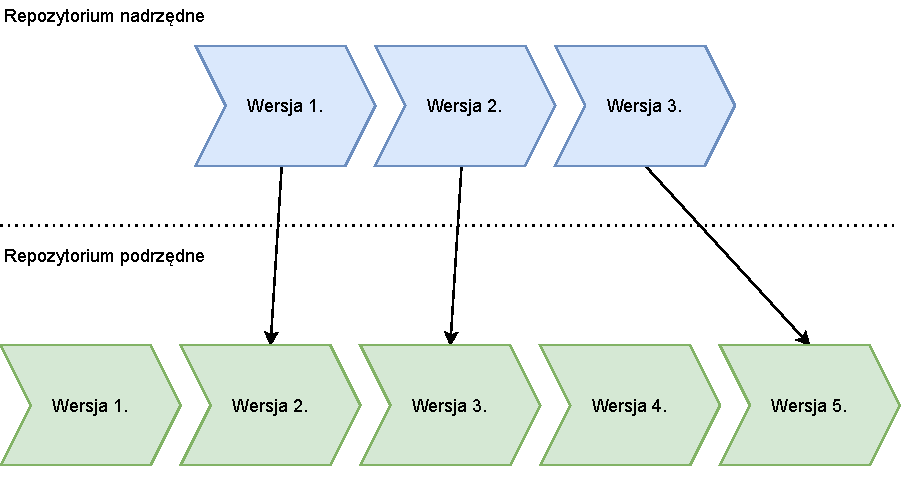
\includegraphics[width=0.9\textwidth]{submodule_links.pdf}
    \caption{Zasada działania submodułów: dowiązanie w~ramach danej wersji repozytorium nadrzędnego wskazuje na konkretną wersję repozytorium podrzędnego.}
    \label{fig:submodules_links}
\end{figure}

\lstinputlisting[
    language=Cmd, 
    caption={Inicjalizacja pełnej struktury projektu jedną komendą.}, 
    label={lst:initialize}
]{4_infrastructure/code_samples/submodules_init.txt}

\subsection{Motywacja do wprowadzenia zmian}
Pomimo wielu aspektów \emph{git submodules}, które bardzo dobrze wpasowały się w~kreowaną przez autorów w~trakcie pracy inżynierskiej strukturę, z~technologią tą związanych jest szereg niedogodności. Pierwszy znaczącym problemem napotkanym w~trakcie pracy z~submodułami było nietypowe zachowanie repozytoriów w~trakcie ich inicjalizacji, a~konkretnie automatyczne odłączanie ich od głównej gałęzi (wynika to z~faktu, iż śledzenie zależności polega w~tym przypadku na zapamiętywaniu identyfikatora konkretnej rewizji, nie zaś informacji o~gałęzi). Co więcej praca z~submodułami wymaga od programisty zwiększonej czujności oraz stosowania dodatkowych zasad, ponieważ więcej jest miejsc na pomyłkę, co może doprowadzić do niepoprawnego działania wykorzystanych narzędzi. Kolejnym problemem napotkanym w~trakcie pracy z~submodułami jest czasochłonność niektórych operacji, w~szczególności aktualizacji repozytorium na samym spodzie drzewa zależności. Zmiana taka wymaga manualnej aktualizacji po kolei każdego z~repozytorium, aż do samej góry tejże struktury, co przedstawia rysunek \ref {fig:submodules_update}. Każda z~aktualizacji przedstawiona na wspomnianym rysunku, to tak na prawdę cztery lub więcej koniecznych do wykonania akcji, do których wliczają się: aktualizacja repozytorium podrzędnego, dodanie wszystkich zmian do rejestru odpowiedzialnego za ich śledzenie, utworzenie nowej wersji repozytorium, opublikowanie nowej wersji na zewnętrznym serwerze.

\begin{figure}[H]
    \centering
    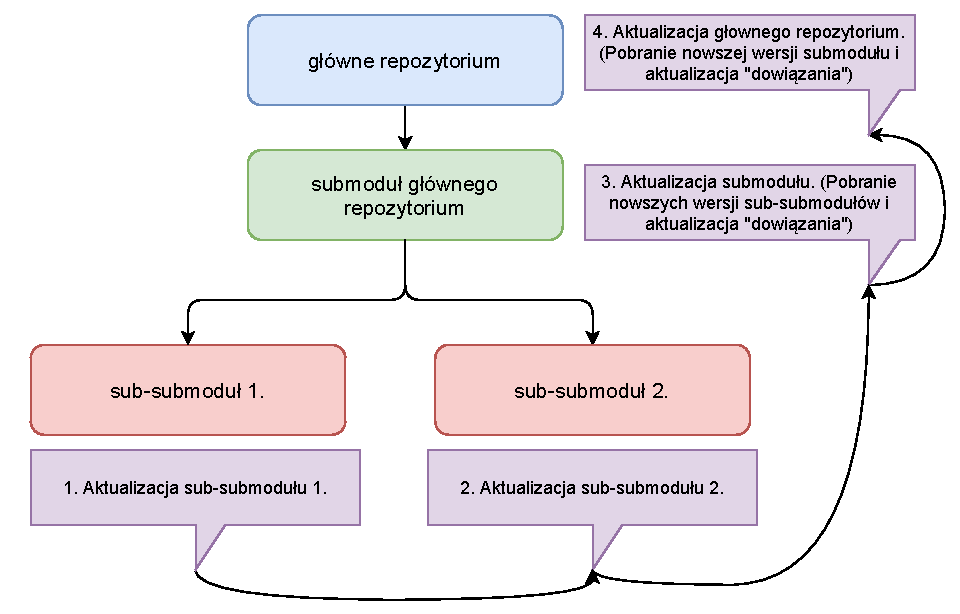
\includegraphics[width=\textwidth]{submodules_update.pdf}
    \caption{Przykładowa architektura oparta o~submoduły z~krokami jakie należy podjąć, aby wprowadzić zmiany na ``najniższym`` poziomie.}
    \label{fig:submodules_update}
\end{figure}


\subsection{Automatyzacja z użyciem dedykowanego narzędzia}
\label{subsec:gitio}
Konieczność wykonywania szeregu powtarzalnych czynności w~celu wprowadzenia oraz propagacji zmian w~poszczególnych modułach projektu GGSS stanowiła problem, który potencjalnie mógłby pochłonąć bardzo znaczącą ilość czasu, możliwego do przeznaczenia na rozwój samego systemu. Dlatego też już w~początkowych tygodniach opisywanych prac autorzy zdecydowali się na przygotowanie, z~wykorzystaniem języka Python, aplikacji \emph{gitio}, której zadaniem było rozwiązanie przedstawionego problemu. Ze względu na to, że metadane technologii Git są bardzo złożone, a~opanowanie zasad wewnętrznego działania tejże technologii wymagałoby bardzo dużo czasu, skorzystano z~dedykowanej biblioteki \cite{gitpython} dostępnej z~poziomu języka Python. Argumenty wejściowe przyjmowane przez \emph{gitio} to:
\begin{itemize}
    \item \lstinline{-h, --help} - pozwala na wyświetlanie informacji o~przeznaczeniu programu oraz przyjmowanych argumentach wraz z~krótkim opisem
    \item \lstinline{-p PATH, --path PATH} - ścieżka do głównego folderu zawierające drzewo repozytoriów do wyrównania
    \item \lstinline{-b BIN, --bin BIN} - ścieżka do aplikacji Git (argument ten jest wymagany jedynie, jeżeli \emph{gitio} nie jest w~stanie automatycznie wykryć Git'a)
\end{itemize}

Przed uruchomieniem aplikacji \emph{gitio} należy uprzednio przygotować repozytoria, które mają zostać poddane procesowy wyrównania. W~tym celu należy wykonać następujące kroki:
\begin{itemize}
    \item sklonować główne repozytorium - \lstinline{git clone <url>}. W~celu poprawnego działania należy sklonować repozytorium z~użyciem klucza ssh.
    \item zainicjalizować i~zaktualizować wszystkie submoduły za pomocą komendy: \\
        \lstinline{git submodule update --init --recursive}
    \item ustawić główną gałąź na każdym z~submodułów za pomocą komendy: \\
        \lstinline{git submodule foreach --recursive "git checkout master"}
\end{itemize}
Zasada działania aplikacji jest stosunkowo prosta, natomiast znacząco ułatwia ona działania z~wielopoziomową strukturą opartą o~\emph{git submodules}. W~pierwszej kolejności \emph{gitio} analizuje strukturę katalogów oraz metadane zawarte w~folderach \lstinline{.git}, dzięki czemu jest w~stanie zapisać w~pamięci zależności między repozytoriami. Następnie przechodząc od samego dołu drzewa zależności, czyli repozytoriów, które nie mają żadnych submodułów, wykonywane są następujące akcje:
\begin{itemize}
    \item aktualizacja rewizji, na które wskazują submoduły do najnowszych dostępnych w~zdalnym repozytorium
    \item utworzenie nowej rewizji z~zaktualizowanymi submodułami
    \item przekazanie nowej rewizji do podłączonego zewnętrznego repozytorium.
\end{itemize}
W~celu zapewnienia bezpieczeństwa \emph{gitio} pozwala na wyrównanie wersji repozytoriów tylko w~przypadku, gdy w~danym repozytorium nie ma żadnych zmian od wykonania ostatniej rewizji. 

Rysunek \ref{fig:gitlab_gitio} przedstawia przykładową rewizję na portalu GitLab utworzoną z~użyciem \emph{gitio}. Wiadomość w~ramach utworzonej rewizji, czyli \emph{Automatic repository update}, wskazuje na wykorzystanie \emph{gitio}. Jedyne zmiany jakie jest w~stanie wprowadzić \emph{gitio}, to aktualizacja rewizji pod-projektu, co również widoczne jest na załączonym rysunku.

\begin{figure}[H]
    \centering
    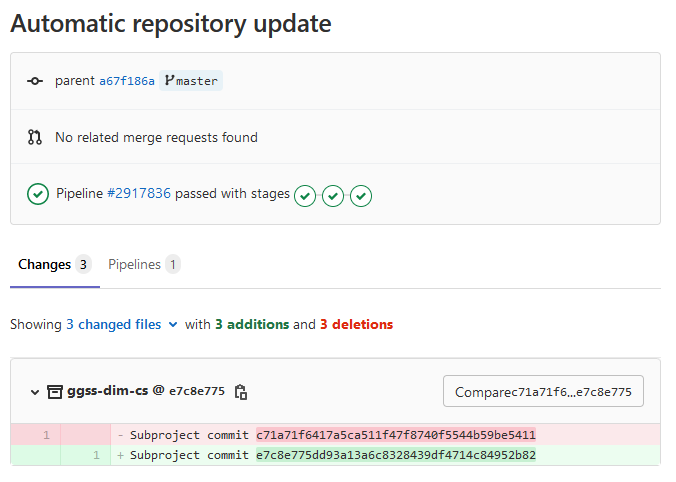
\includegraphics[width=\textwidth]{gitio_gitlab.png}
    \caption{Przykładowa rewizja utworzona z~użyciem \emph{gitio}.}
    \label{fig:gitlab_gitio}
\end{figure}


\subsection{Dokumentacja sposobu pracy z submodułami}
Ze względu na to, że praca z~repozytoriami posiadającymi submoduły wymaga poświęcenia dodatkowej uwagi oraz stosowania specyficznych praktyk, autorzy postanowili przygotować stosowną dokumentację, w~formie plików \emph{README} umieszczonych w~repozytorium \emph{ggss-aux}. Jej stosowanie pozwala na uniknięcie poważnych błędów, które mogłyby doprowadzić do niepoprawnego działania systemu kontroli wersji.

Dokumentacja została podzielona na trzy części. Pierwsza z~nich odnosi się do poprawnej inicjalizacji repozytoriów z~wielopoziomowymi submodułami. Poniżej zaprezentowane zostało krótkie streszczenie zawartych tam informacji:
\begin{itemize}
    \item W~pierwszej kolejności należy sklonować odpowiednie repozytorium z~zewnętrznego serwera. W~celu ułatwienia pracy z~submodułami należy akcję tę wykonać za pomocą protokołu SSH wraz z~przypisanym kluczem. Pozwala to uniknąć wielokrotnego wpisywania loginu oraz hasła przy każdorazowym klonowaniu submodułów. Przykładowa komenda dla repozytorium \lstinline{ggss-all} wygląda następująco: \lstinline{git clone ssh://git@gitlab.cern.ch:7999/atlas-trt-dcs-ggss/ggss-all.git}.
    \item W~ramach poprzedniego kroku sklonowane zostało jedynie główne repozytorium, brak jest zawartości katalogów z~submodułami. Ich inicjalizacja powinna zostać wykonana komendami \lstinline{git submodule init} oraz \lstinline{git submodule update}, natomiast w~celu przyspieszenia tego procesu można wykonać jedną komendę, a~mianowicie \lstinline{git submodule update --init --recursive}. Właśnie taka komenda polecana przez przez autorów do pracy z~projektem GGSS.
    \item Ze względu na sposób działania submodułów, przed dokonaniem zmian należy jeszcze zmienić gałęzie we wszystkich submodułach na gałąź docelową. Domyślnie inicjalizacja submodułów powoduje, że znajdują się one w~stanie \lstinline{detached HEAD}, co oznacza odwołanie do konkretnej rewizji, a~nie gałęzi. W~celu dokonania zbiorczego ustawienia gałęzi należy wykonać komendę \lstinline{git submodule foreach --recursive "git checkout master"}
\end{itemize}

Kolejna część dokumentacji odnosi się do porad i~dobrych praktyk, które należy stosować pracując z~infrastrukturą repozytoriów opartą o~submoduły. Ostatnią częścią dokumentacji jest natomiast krótki opis, w~jaki sposób propagować zmiany w~całym projekcie GGSS. Propagacja odbywa się za pomocą wyrównania wersji wskazywanych przez submoduły, a~zatem przez odpowiednie skorzystanie z~\emph{gitio}. Więcej szczegółów jak skorzystać z~\emph{gitio} oraz warunków jakie należy spełnić zostały opisane w~sekcji \ref{subsec:gitio}. Treść przygotowanej dokumentacji załączona została do niniejszej pracy w~formie dodatku \ref{sec:working-with-git-sudmobules}.
